\chapter[Discrete symmetry tests with odd operators in ortho-positronium decays]{Discrete symmetry tests with odd operators in ortho-positronium decays}\label{chapter:test_jpet}

Although the \Ts,~\CPs~and~\CPTs~symmetries have been investigated thoroughly in a multitude of physical systems during the past half of a century, experimental results on their tests in purely leptonic systems have been scarce~\cite{Arbic:1988pv,Skalsey:1991vt,cp_positronium,cpt_positronium}. Among the latter, the positronium exotic atoms constitute a likely candidate for precise searches of discrete symmetries' violations~\cite{Bernreuther:1988tt}. The most recent experimental attempts, testing the \CPs~and \CPTs~symmetries in the ortho-positronium decays, both obtained null results with a precision at the level of $10^{-3}$~\cite{cp_positronium,cpt_positronium}. Possible searches for symmetries' violation in the positronium decays are only limited by photon-photon final state interactions which may cause false asymmetries~\cite{Bernreuther:1988tt,Arbic:1988pv} and by weak interactions~\cite{sozzi}. These effects are, however, expected at the levels of $10^{-9}$ and $10^{-14}$, respectively, which leaves a vast space still to be explored. Pushing the presently obtained precision limits in the discrete symmetry studies with o-Ps atoms is one of the aims of the \jpet/ experiment. This Chapter discusses the planned measurements with a special emphasis on their dependency on the trilateration-based reconstruction technique for o-Ps$\to 3\gamma$ decays, presented in~\cref{chapter:gps} of this Thesis.

\section{Properties of the ortho-positronium atoms}
Positronium is a bound state of an electron and a positron, which may be formed prior to their annihilation. Having a reduced mass only twice smaller than a hydrogen atom, it has a similar energy level structure and is thus often referred to as an exotic atom. While being an eigenstate of the parity operator like atoms, positronium is also symmetric under charge conjugation operation as a particle-antiparticle system. As the positronium spin is a linear combination of electron and positron spins, four possible states may be formed depending on their orientation~\cite{Harpen:2003zz}:
\begin{eqnarray*}
  \ket{S=1,S_Z=1} &=& \ket{\uparrow}\ket{\uparrow},\\
  \ket{S=1,S_Z=0} &=& \frac{1}{\sqrt{2}}\left[\ket{\uparrow}\ket{\downarrow}+\ket{\downarrow}\ket{\uparrow}\right],\\
  \ket{S=1,S_Z\!=\!-1} &=& \ket{\downarrow}\ket{\downarrow},\\
  \ket{S=0,S_Z=0} &=& \frac{1}{\sqrt{2}}\left[\ket{\uparrow}\ket{\downarrow}-\ket{\downarrow}\ket{\uparrow}\right],
\end{eqnarray*}
where $\ket{\uparrow}$ and $\ket{\downarrow}$ denote $S_z=+\frac{1}{2}$ and $S_z=-\frac{1}{2}$ for a single electron or positron. The three states with $S=1$ constitute a triplet known as ortho-positronium~(\ops/) whereas the $S=0$ singlet state is referred to as para-positronium~(p-Ps). In the ground state with $l=0$, the charge conjugation parity of such a system depends on the spin as $({-1})^S$ and is therefore different for para- and ortho-positronium. As the electromagnetic interactions conserve charge parity, the allowed final states of para-positronium annihilation must contain an even number of photons ($C=(-1)^n$ for a system of $n$ photons) whereas o-Ps can only annihilate into an odd number of photons. In practice, final states with larger photon numbers are suppressed by few orders of magnitude and the positronium annihilations are dominated by p-Ps$\to 2\gamma$ and o-Ps$\to 3\gamma$~\cite{Harpen:2003zz}.

The difference of allowed decays is also a reason for much larger mean lifetime of ortho-positronium atoms due to a smaller available phase space and smallness of the fine structure constant ($\approx$1/137). In vacuum, the lifetimes of ortho and para states amount to~\cite{PhysRevLett.72.1632,PhysRevLett.90.203402,JINNOUCHI2003117}:
\begin{eqnarray*}
  \tau_{\text{p-Ps}} &\approx& 0.125\ \text{ns}, \\
  \tau_{\text{o-Ps}} &\approx& 142\ \text{ns}.
\end{eqnarray*}

Such a lifetime discrepancy makes it possible to distinguish the p-Ps and \ops/ states experimentally if the positronium creation and decay time can be measured. The former may be estimated e.g.\ when positronia are created with $e^+$ from a source in which $\beta^+$ emission results is creation of a nucleus in an excited state, where the prompt de-excitation photon provides a time signal approximately corresponding to the positronium creation~\cite{daria_epjc}.

\section{Symmetry tests with angular correlations in o-Ps$\to 3\gamma$}
\label{sec:ops_operators}
Ortho-positronium annihilations into three photons allow for experimental searches of discrete symmetry violations which could be manifested by specific angular correlations in the events' topology~\cite{Bernreuther:1988tt}. To measure such asymmetries, several operators can be constructed using four vectors measurable in a single annihilation event: momenta of the three photons $\vec{k_i},\ i=1,2,3$ and spin $\vec{S}$ of the decaying ortho-positronium atom. As depicted in~\fref{fig:ops_decay_scheme}, the photons' momentum vectors are constrained by momentum conservation to lie in a single plane, and are not correlated with the \ops/ spin. In order to distinguish the three photons, they can be ordered by decreasing energy so that $|\vec{k_1}| > |\vec{k_2}| > |\vec{k_3}|$.

\begin{table}
  \centering
  \caption{Operators constructed with photons' momenta and ortho-positronium spin $\vec{S}$ which can be used for discrete symmetry tests in the o-Ps$\to 3\gamma$ decays. For each listed symmetry, $+$ and --- indicate that the operator is even or odd, respectively.\label{tab:jpet_operators}}
  \begin{tabular}[h!]{cp{3em}p{3em}p{3em}p{3em}p{3em}}
    \toprule
    operator & C & P & T & CP & CPT \\
    \midrule
    ${\vec{S} \cdot \vec{k_1}}$ & + & --- & + & --- & ---\\      
    ${\vec{S} \cdot (\vec{k_1}\times\vec{k_2})}$ & + & + & --- & + & ---\\
    $({\vec{S} \cdot \vec{k_1})(\vec{S} \cdot (\vec{k_1}\times\vec{k_2})})$ & + & --- & --- & --- & +\\
    \bottomrule
  \end{tabular}
\end{table}

\tref{tab:jpet_operators} lists three operators which can be built with the aforementioned vectors, along with their parity with respect to chosen symmetry operations~\cite{moskal_potential}.
%
% @TODO: sprawdzić czy to jest prawda w ogóle
%
The considerations for the expectation value of an operator odd under time reversal from Equations~\ref{eq:rel_any_operator}--\ref{eq:expectation_value_any_operator} can be applied to other symmetry transformations (in case of \CPs, which is unitary, the hermicity of the operator O is not required). As a result, any of the operators from~\tref{tab:jpet_operators} which is odd under a certain symmetry transformation can be used to construct a test of this symmetry by searching for the operator's non-vanishing expectation value.

\begin{figure}[h!]
  \centering
  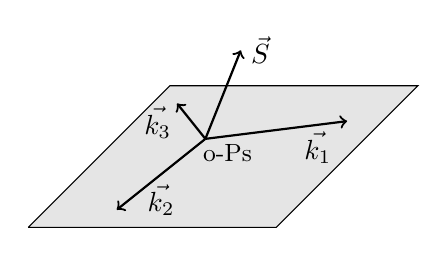
\begin{tikzpicture}[scale=0.45]
    % 
    \filldraw[fill=gray!20] (-5,4) -- (2,4) --  (6,8) -- (-1,8) -- (-5,4);
    % 
    \draw[black,thick,->] (0,6.5) node[black,yshift=-5,xshift=8]{\small o-Ps} -- (1,9) node[anchor=west] {$\vec{S}$};
    % 
    \draw[black, thick,->] (0,6.5) -- (4,7)node[midway, below,xshift=15,yshift=3] {$\vec{k_1}$};
    \draw[black, thick,->] (0,6.5) -- (-0.8,7.5)node[yshift=-7.0,xshift=-7.0] {$\vec{k_3}$};
    \draw[black, thick,->] (0,6.5) -- (-2.5,4.5)node[midway, below] {$\vec{k_2}$};
  \end{tikzpicture}
  \caption{Vectors in an o-Ps$\to 3 \gamma$ event (in the \ops/ frame of reference) used to construct the operators listed in~\tref{tab:jpet_operators}. The photons' momentum vectors are ordered by magnitude so that $|\vec{k_1}| > |\vec{k_2}| > |\vec{k_3}|$. $\vec{S}$ denotes the spin of the decaying positronium.}\label{fig:ops_decay_scheme}
\end{figure}

As the aforementioned operators correspond to particular angular correlations in the \ops/$\to 3\gamma$ events, their non-zero mean value can be experimentally sought in the following asymmetry:
\begin{equation}
  A = \frac{N_+ - N_-}{N_+ + N_-},
\end{equation}
where $N_+$ and $N_-$ respectively are the numbers of observed events with a positive or negative value of a certain correlations, e.g.\ for the T-odd operator ${\vec{S} \cdot (\vec{k_1}\times\vec{k_2})}$, $N_-$ will be the count of events with the decay plane normal vector $\vec{k}_1\times\vec{k}_2$ anti-parallel to the \ops/ spin.

%%% Local Variables:
%%% TeX-master: "../main"
%%% End: